\subsection{Sorting}

\begin{frame}[fragile]
\frametitle{Sorting}

\begin{figure}[h]
\centering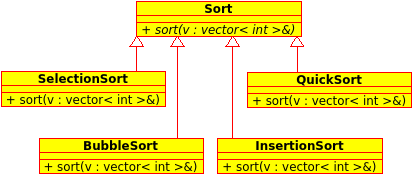
\includegraphics[scale=0.7]{img/sorting.png}
\caption{Sorting Framework}
\end{figure}

\subsubsection{Abstract class Sort}
The implementation of different sorting algorithms should be based on
the abstract Sort class as given in the following diagram:

\end{frame}

\begin{frame}[fragile]
\frametitle{Sorting}
{\small
\lstinputlisting{code/sort/sort.h}
}

\end{frame}

\begin{frame}[fragile]
\frametitle{Bubble Sort}
{\tiny
Bubble sort is a simple sorting algorithm that repeatedly steps through the list to be sorted,
compares each pair of adjacent items and swaps them if they are in the wrong order.
The pass through the list is repeated until no swaps are needed, which indicates that the
list is sorted. 
\verbatiminput{bubblesort.txt}
Runtime: $O(n^2)$
}
\end{frame}

\begin{frame}[fragile]
\frametitle{Selection Sort}
{\tiny
Selection sort divides the input list into two parts: the sublist of items already sorted,
which is built up from left to right at the front (left) of the list, and the sublist of items
remaining to be sorted that occupy the rest of the list. Initially, the sorted sublist is empty and the
unsorted sublist is the entire input list. The algorithm proceeds by finding the smallest element in the
unsorted sublist, exchanging (swapping) it with the leftmost unsorted element (putting it in sorted order),
and moving the sublist boundaries one element to the right.
\verbatiminput{selectionsort.txt}
Runtime: $O(n^2)$
}
\end{frame}

\begin{frame}[fragile]
\frametitle{Insertion Sort}
{\tiny
Insertion sort iterates, consuming one input element each repetition, and growing a sorted output list.
Each iteration, insertion sort removes one element from the input data, finds the location it belongs within
the sorted list, and inserts it there. It repeats until no input elements remain.
\verbatiminput{insertionsort.txt}
Runtime: $O(n^2)$
}
\end{frame}

\begin{frame}[fragile]
\frametitle{Quick Sort}
\begin{figure}[h]
\centering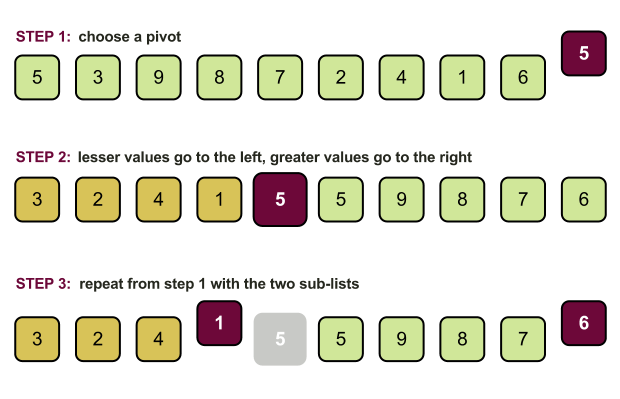
\includegraphics[scale=0.3]{img/quicksort_new.png}
\caption{Quicksort Algorithmus}
\end{figure}
Runtime: $O(n \cdot log(n))$
\end{frame}

\begin{frame}[fragile]
\frametitle{Quick Sort}
Worst Case: Array is already sorted.
\begin{figure}[h]
\centering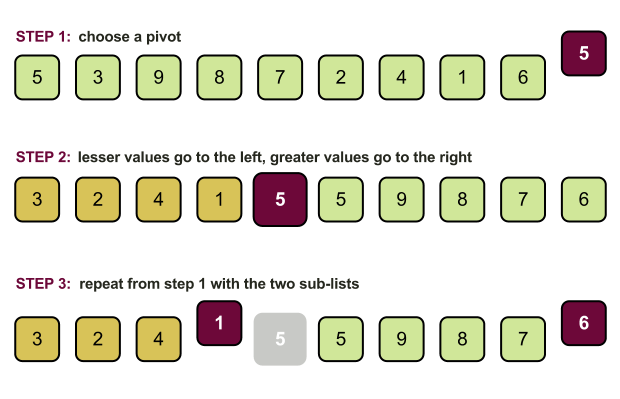
\includegraphics[scale=0.3]{img/quicksort_new.png}
\caption{Quicksort Algorithm Worst Case}
\end{figure}
Runtime: $O(n^2)$
\end{frame}

\begin{frame}[fragile]
\frametitle{Randomized Quick Sort}
Do not take the last element as pivot element, just choose
the pivot element randomly from all available elements.\\
Change the last element with the pivot element, therefore
the code developed before is still usable.
Runtime: $O(n \cdot log(n))$
\end{frame}

\begin{frame}[fragile]
\frametitle{Merge Sort}
\begin{figure}[h]
\centering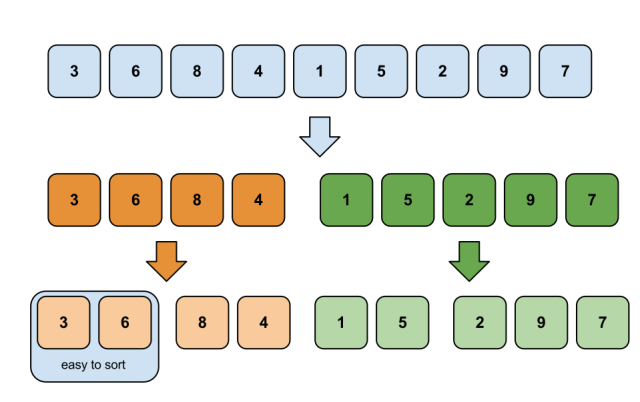
\includegraphics[scale=0.3]{img/mergesort_new.png}
\caption{Merge Sort Algorithm}
\end{figure}
Runtime: $O(n \cdot log(n))$
\end{frame}

\begin{frame}[fragile]
\frametitle{Performance}
Sorting of 100000 elements:
\begin{itemize}
\item Selection Sort: 9.27952s
\item Bubble Sort: 25.1975s
\item Quick Sort: 0.027657s
\item Merge Sort: 0.029053s
\item STL Sort: 0.009174s
\end{itemize}
\end{frame}

